\documentclass[12pt]{article}

\usepackage{cite}
\usepackage{listings}
\usepackage{times}
\usepackage{color}
\usepackage{url}
\usepackage{multirow}
\usepackage{multicol}
\usepackage{enumitem} % Use for enumerating A, B, C etc...
\urlstyle{same} % Used for formatting formatting url footnotes
\usepackage{fancyhdr} % Header
%\usepackage[table]{xcolor}% http://ctan.org/pkg/xcolor
\usepackage[table,xcdraw]{xcolor} % helps to format TOC
\usepackage{soul} % highlighting
%\usepackage{pgfgantt} % Project timeline
\usepackage[titletoc,toc,title]{appendix} % Need for appendix, page numbering
\usepackage{tikz}
\usetikzlibrary{calc,arrows.meta,fit,positioning}
%\usepackage{amssymb,graphicx} % Events and milestones
\usepackage{amsmath}
\usepackage{mathtools}
%\usepackage{bbm}
\usepackage{amssymb}
\usepackage{lastpage}

%\usepackage{algorithm}
%\usepackage[noend]{algpseudocode}



\usepackage{framed}		% Allows drawing text boxes
\usepackage{pgfgantt}
\usepackage{rotating}
\usepackage[graphicx]{realboxes}
\usepackage{pgf-umlsd}
\usepackage{tikz}




\usepackage{xspace} % Needed for et al.
\newcommand{\ie}{\emph{i.e.,}\xspace}
\newcommand{\eg}{\emph{e.g.,}\xspace}
\newcommand{\etc}{etc.\xspace}
\newcommand{\etal}{\emph{et~al.}\xspace}  

% Page margins etc....
\usepackage[bottom=1in, left=1in, right=1in, top=1in]{geometry} % Should all be 1
%.85

\usepackage[english]{babel}
\usepackage[utf8x]{inputenc}
\usepackage{graphicx}
%\usepackage{wrapfig}
%\usepackage{lipsum}
%\usepackage{pgfgantt}

%\usepackage{minted} % Side by side code

\newcommand{\todo}[1]{\textcolor{cyan}{\textbf{[#1]}}}
\newcommand{\dan}[1]{\textcolor{blue}{{\it [Dan: #1]}}}
\newcommand{\qi}[1]{\textcolor{red}{{\it [Qi: #1]}}}
\newcommand{\alex}[1]{\textcolor{green}{{\it [Alex: #1]}}}
\newcommand{\travis}[1]{\textcolor{brown}{{\it [Travis: #1]}}}

%%% Start column formatting
% Note: In overleaf sometimes columns fail to render. Check on PDF Output
\newcolumntype{L}[1]{>{\raggedright\arraybackslash}m{#1}} % raggedright= align left
\definecolor{Gray}{gray}{0.80} % the lower the #, the darker it gets
%%% End Table formatting

\newcommand{\descStep}[2]{\noindent \textbf{#1: } #2}
\newcommand{\objective}[3]{\vspace{2mm} \noindent \textbf{{Objective #1 - #2: }} #3} % Describing objectives

%%%% Start toggling showing/hiding some information
\newif\ifShowAll
\ShowAlltrue % Display All Info
%\ShowAllfalse % Hide Some Info


% Using Recurrent Neural Networks to Account for Tactic Volatility and Improve the Decision-Making Process of Autonomous Systems 

% Accounting for Tactic Volatility in Self-Adaptive Systems Using % Accounting for Tactic Volatility: Improving Autonomous System Decision-Making Using Evolving Recurrent Neural Networks

%Accounting for Tactic Volatility: Improving Autonomous System Decision-Making Using Evolving Recurrent Neural Networks and Multi-Armed Bandits

% Accounting for Tactic Volatility: Improving Autonomous System Decision-Making Using Evolving Recurrent Neural Networks and Multi-Armed Bandits

\newcommand{\Title}{Accounting for Tactic Volatility: Improving Decision-Making in Autonomous System Using Evolving Recurrent Neural Networks and \hl{Multi-Armed Bandits}}

\newcommand{\shortTitle}{Accounting for Tactic Volatility in Autonomous Systems} % Used in the heading just so it fits

\newcommand{\CallNumber}{W911NF-17-S-003} % BAA Number
\newcommand{\CallName}{XXXX}
%\newcommand{\BAANumber}{N00421-18-S-0001}

\usepackage{fancyhdr} % Header
\pagestyle{fancy}
\lhead{\emph{\shortTitle}}
%\rhead{Krutz (RIT)}
\rhead{Krutz: dxkvse@rit.edu}
%\lhead{\shortTitle}
%\rhead{}


%\setlength\cftparskip{-.7pt} %% Table of contents spacing
%\setlength\cftbeforechapskip{0pt}

\begin{document}

\begin{titlepage}

\newcommand{\HRule}{\rule{\linewidth}{0.3mm}} % Defines a new command for the horizontal lines, change thickness here

%%%%%%% Start new Title format


%% DK: I am not sure if we should have this
%\noindent\large \CallName, \CallNumber\\[.20cm] % Call Name

%  \textsc{\Large White Paper Submission\dan{update page with required information}}\\[0.5cm] % Major heading

%\noindent\large \CallNumber\\[.20cm] % Call Name


\begin{center}
  \textsc{\Large White Paper Submission}\\[0.5cm] % Major heading such as course name
  \textsc{\large \CallNumber}\\[1.5cm]   %% Fix this
\end{center}

%\noindent \LARGE \textbf{\Title}\\[.10cm] % Title
\noindent \Large \textbf{\Title}\\[.10cm] 


\noindent \large  \underline{\textbf{Technical Proposal}}\\ [.15cm] 

\begin{tabular}{ L{50mm} L{100mm} }

%\normalsize \textbf{Technical Proposal:} & \normalsize  \CallName, \CallNumber  \\

%\noindent\large Technical Proposal: N00174-18-0001\\[.20cm]
%\noindent\large NEC Technical POC: \\[.20cm]
%\noindent\large Topic Number: \\[.20cm]

%\normalsize \textbf{BAA Number:} & \normalsize \CallNumber  \\
%\normalsize \textbf{Proposed Title:} & \normalsize  \Title  \\ 
\normalsize \textbf{Research opportunity area:} & \normalsize  Artificial Intelligence and Machine Learning  \\ 
% Research opportunity area of interest

\normalsize \textbf{Technical POC/PI:} & \normalsize  Dr. Daniel Krutz \\
 & \vspace{-2mm} \normalsize Department of Software Engineering
 \\

   & \vspace{-4mm} \normalsize 152 Lomb Memorial Drive \\
   & \vspace{-6mm} \normalsize Rochester, NY 14623 \\
   & \vspace{-8mm} \normalsize Phone: (585) 475-2896 \\
   & \vspace{-10mm} \normalsize Email: dxkvse@rit.edu \\
   
   
   
%   \normalsize \textbf{Co-PI:} & \normalsize  Dr. Daniel Krutz \\
% & \vspace{-2mm} \normalsize Department of Software Engineering
 \\

%   & \vspace{-4mm} \normalsize 152 Lomb Memorial Drive \\
%   & \vspace{-6mm} \normalsize Rochester, NY 14623 \\
%   & \vspace{-8mm} \normalsize Phone: (585) 475-2896 \\
%   & \vspace{-10mm} \normalsize Email: dxkvse@rit.edu \\
   
   
   
   
   

%\vspace{-6mm}\normalsize \textbf{Administrative POC:} & \vspace{-6mm} \normalsize Ms. Laura Kleiman \\

%%   & \vspace{-8mm} \normalsize Senior Research Administrator  \\
%   & \vspace{-9mm} \normalsize Sponsored Research Services  \\
%   & \vspace{-11mm} \normalsize Rochester Institute of Technology  \\
%   & \vspace{-13mm} \normalsize University Services Center, Suite 2400  \\
%   & \vspace{-15mm} \normalsize 141 Lomb Memorial Drive, Rochester, NY 14623-5608   \\
%   & \vspace{-17mm} \normalsize Rochester, NY 14623-5608  \\
%   & \vspace{-19mm} \normalsize Phone: (585)-475-2262  \\
%%   & \vspace{-22mm} \normalsize Facsimile: (585)-475-2262  \\
%   & \vspace{-21mm} \normalsize Email: ljksrs@rit.edu  \\


%BAA Number, proposed title, research opportunity area of interest, contracts and technical points of contact, telephone number, facsimile number, and E-mail address


\end{tabular}

 \end{titlepage}

\cfoot{\thepage}
\pagenumbering{alph} % Start roman numbering
\setcounter{tocdepth}{1} % Show sections

\cfoot{} % Leave blank


%%%%% TOC - Start
%\renewcommand\contentsname{Table of Contents}
%\tableofcontents
%\listoffigures
%\listoftables
%\newpage

%%%%% TOC - End


\setcounter{page}{1}
\pagenumbering{arabic} % Switch to normal numbers

%\cfoot{\thepage\ of \pageref{LastPage}}
\fancyfoot[C]{Page~\thepage~of~\pageref{lastpage}}


\section{Introduction}

% ? Mention ASE paper someplace?

% Should bandits in title be plural









%The proposed work will enable autonomous systems to \textbf{better account for uncertainty} and \textbf{volatility and to operate in real world, volatile environments with/using small amounts of prior data}. \dan{modify this a bit to include the benefits of the ML stuff}

%\textbf{The proposed work will enable autonomous systems to operate in real-world, volatile environments using small amounts of prior data through the use of Recurrent Neural Networks (RNNs).}

%\textbf{The proposed work will enable autonomous systems to rapidly adapt to new and volatile environments using online evolution of recurrent neural networks (RNNs) to account for tactic volatility.}


% DK: ? Should we add something about tactics in here as well?
\textbf{The proposed work will enable autonomous systems to rapidly adapt to new and volatile environments using online evolution of recurrent neural networks (RNNs) and a multi-armed bandit approach.}





% DK: This is ok, but doesn't mention anything specifically regarding tactic volatility


%\dan{Add in the type of learning model that we will use, RNN - Make sure that it is introduced and that we briefly describe how and why it will be beneficial}
%\dan{If a large contribution of the project will be in learning, it likely wouldn't be a bad idea to make that more clear in the introduction/opening statement.}

Autonomous systems frequently operate in new and volatile environments that contain large amounts of uncertainty and variability. Therefore, it is imperative that autonomous systems be enabled to quickly adapt, and appropriately manage uncertainty and variability to remain effective, resilient and retain the ability to accomplish mission and system objectives. \emph{Tactics} are actions performed by autonomous systems to respond to changes in their environment or to achieve objectives. Tactic examples include reducing non-essential functionality on a UAV when battery levels are low, or the provisioning of an additional virtual machine in a web farm when the workload reaches a specific threshold. The decision-making components in autonomous systems rely upon accurate information to select the tactic(s) that will result in the most optimal outcome. Real-world systems will frequently encounter \emph{tactic volatility}, which is any rapid or unpredictable change that exists within the attributes of a tactic. For example, both tactic latency and cost may be highly volatile depending on the system's surrounding environment. A tactic of transmitting data could take longer than expected due to network congestion, or a tactic of utilizing an external resource could be more expensive due to a volatile variable pricing structure. 

The anticipated latency and cost of a tactic is frequently a significant concern in the system's decision-making process, as they can impact which tactic(s) are selected and when they are invoked. Unfortunately, state-of-the-art decision-making processes in self-adaptive systems do not account for tactic volatility~\cite{Krutz_ase_2019, moreno2017adaptation}. This limitation can be highly problematic, adversely impacting the efficiency and effectiveness of the system. For example, a tactic may be statically defined to always take two seconds, leading the system to believe that it should begin the execution of this tactic two seconds before it is needed. However, if the tactic consistently takes longer than two seconds and the system cannot learn to account for this additional latency, then the tactic will frequently not be ready when needed.\dan{proofread}


%For example, a system may expect a tactic to take two seconds to complete its execution, when in reality it has been observed to consistently take longer; thus leading to situations when the tactic is not available when needed since it is invoked too late.


%For example, a system may execute a tactic too late to be effective if it assumes that the tactic will always take two seconds to conduct, when in reality it has been observed to consistently take longer.\dan{proofread this}

%moving a physical component in a UAV could be more expensive due to mechanical problems.








% What tactic volatility is
% Its negative impact on the overall system - Why it is detrimental
% How current systems do not account for tactic volatility




%Information gathered by these autonomous systems come from various physical and software sensor streams that provide time series data at various intervals. This tactical data can be potentially unreliable and volatile, especially when operating in new or uncontrolled environments. Inaccurate information used in the decision-making process will frequently lead to decisions producing less than optimal benefit, or even undesired outcomes. Unfortunately, state-of-the-art decision-making processes in autonomous systems do not account for uncertainty and variability in the attributes of the tactic~\cite{moreno2017adaptation, Moreno:2017:CMP:3105503.3105511, camara2016analyzing}.

%Some forms of tactic volatility include latency, cost, dependability and availability of the tactic.
% DK: Might be a good idea to define these someplace
 %For example, the cost and latency necessary to perform a tactic operation can be impacted by innumerable internal and external events. 
A robust decision-making and prediction mechanism is needed to enable autonomous systems to better anticipate and account for tactic volatility to reduce uncertainty and to operate in new and dynamic environments. \ul{This pioneering research will develop a \emph{Tactic Volatility Aware} (TVA) solution that will enable autonomous systems to better account for volatility, especially when operating in new and variable environments with limited amounts of historical data.} This will be accomplished through a novel online neuro-evolution strategy that will progressively design recurrent neural networks (RNNs) for predicting tactical data. This will enable these RNNs to quickly adapt to new and dynamic sensors and environments via transfer learning, while simultaneously being able to detect and ignore anomalous, unreliable and potentially adversarial inputs. A multi-armed bandit component will be integrated into the system's decision-making process to better enable the system to account for tactic volatility and reduce tactic uncertainty. This component will direct the system's tactic uncertainty reduction (`explore') and execution (`exploit') operations.

% This component will direct the system's tactic uncertainty reduction operations (`explore' and `exploit' operations 

% 


%\hl{A multi-armed bandit component will be combined with the system's decision-making process to enable the system to reduce uncertainty regarding the volatility of the tactic.}

% A multi-armed bandit component will be integrated into the system's decision-making process to better enable the system to account for tactic volatility and reduce tactic uncertainty.

 


%\hl{A multi-armed bandit approach will be combined with the system's decision-making process to help optimize the tactic-based decisions, especially when tactics contain uncertainty and the confidence of tactic predictions are low.}

% DK: Should we state the type of approach that we will use? (\eg Epsilon-Greedy, Upper Confidence Bound, Bayesian)



%optimize

% help optimize the tactic-based decisions, especially when tactics contain uncertainty and the confidence of tactic predictions are low.


%enable it to better account or uncertainty and volatlity with the tactics.\dan{how}

%These will predict data from tactical sensor streams, enabling autonomous systems to swiftly adapt to different available sensor streams and environments, as well as detect and ignore anomalous, unreliable and potentially adversarial sensor inputs. The proposed TVA framework will address the following crucial challenges and limitations currently faced by autonomous systems:




%Making well-informed, adaptive tactical decisions relies on accurate forecasts of the various sensor streams available to the autonomous system. Prior work by the PIs has shown that utilizing a novel parallel neuro-evolution technique can find more accurate recurrent neural network (RNN) structures for time series data prediction faster than training traditional fixed layer architectures in a sequential manner~\cite{desell-exalt-coal-2019}. We propose to expand this neuro-evolution technique to allow for the automated design of generative RNNs to account for sensor uncertainty and to evolve existing RNNs to swiftly account for modified sensor inputs.

%1. We can evolve RNNs as generative models, where the RNN can predict all expected future inputs from sensors. If one or more inputs are off we can utilize predicted values for predictions instead of actual values in the case of sensor damage, degradation or inaccuracies due to a new or uncontrolled environment.

%2. The sensors available to an autonomous system may change over time due to damage or acquisition of new technologies (?components?). Instead of designing and training entirely new RNNs every time a sensor becomes unavailable or available, we can continue to use it but drop out unused/broken sensors and evolve new connections for new sensors, continuing the neuro-evolution process from a previously well trained RNN on that system.  This will allow swift transfer of previous knowledge to the new set of sensors.



We propose to expand upon current state-of-the-art techniques in several ways to facilitate the use of autonomous systems in new and volatile environments:%\dan{add MAB for this?}

\begin{enumerate}[noitemsep]

%	\item The proposed process must enable the autonomous system to more effectively account for uncertainty and variability in its operating environment. 


    \item The proposed framework will swiftly adapt to operations in new, uncontrolled environments, or to changes in sensory inputs due to damage or acquisition of new components.
    
    \item The framework will provide metrics for both confidence of predictions as well as variance of parameters used for tactical decision making.
    
    
%        \item The framework will support systems in learning more information about tactics - MAB?\dan{? remove}


    %\item The framework will provide measures of certainty to a system's sensory input to account for damage or adversarial activity. \dan{can this be removed/integrated into the above item? The both refer to confidence/certainty}
    
    
    %\hl{The calculated historical variance will be included into the decision-making process}\dan{fix}
    
    % For future submissions consider how a human could make use of this certainy in a human/paired team

%	\item When prior mission data is available, the system should incorporate this information into its decision-making process.

	\item The proposed work will support systems in better acting proactively to ensure that specifications defined in the \emph{Service Level Agreement} (SLA) are adhered to.

	\item To support its inclusion a wide-range of existing systems, the proposed framework will easily integrate into existing autonomous decision-making processes and strategies such as MAPE-K~\cite{kephart2003vision} and Rainbow~\cite{garlan2004rainbow}.

\end{enumerate}

The proposed TVA solution is the first that enables autonomous systems to account for \emph{Tactic Volatility}. Through the novel use of online neuro-evolution to adapt RNNs, TVA may be quickly applied to new sensor platforms and learn in new environments with limited amounts of historical data. This will enable the autonomous system to operate in new environments and react to new and unpredictable scenarios while enhancing system resiliency.\dan{is this redundant?}

%%%%%%%
%To the best of our knowledge, the proposed TVA solution is the first that enables autonomous systems to account for \emph{Tactic Volatility}. By using an online neuro-evolution to adapt RNNs, TVA will be able to swiftly applied to new sensor platforms as well as learn in new environments with limited amounts of historical data, thus supporting the autonomous system to operate in new environments and to better react to new and unforeseen situations.\dan{clean this section up}\dan{Add a few more words about the learning solution and why it is good}

% The benefits our work can have on a variety of self-adaptive/autonomous systems
% Why RNN will be a useful solution

% 


\subsection{Motivating Example}
\label{sec: motivatingexample}

% If there is space, add something in about how the confidence/variance could impact the decision

\noindent\textbf{Motivating Example:} The goal of a cloud-based, self-adaptive system~\cite{moreno2017adaptation} is to maximize utility while minimizing cost. An SLA defines the target response time ($T$) and how utility ($U$) is calculated. %The system incurs penalties if the target response time is not met and accrues rewards for meeting the target average response time against the measurement interval. %In this scenario, the cost is directly proportional to the number of servers used. 
The average response rate is $a$, the average response time is $r$, the maximum request is $k$, and the length of each interval is defined as $\tau$. Provided content is reduced as necessary using a dimmer value, ($d$). Optional content has reward of ($R_O$) which produces a higher reward than mandatory content ($R_M$). Cost ($C$) could be the monetary or energy cost:

\begin{equation} \label{eq: motivatingExample}
	U = \left\{ \begin{array}{rl}
 	(\tau a (dR_O+(1-d)R_M)/C~~~~r\leq T \\ 
  	(\tau \min (0,a-k)R_O)/C~~~~r> T 
       \end{array} \right.
\end{equation}

This system can account for increases in user traffic using two tactic options: (I) reducing the proportion of responses that include the optional content (dimmer), and (II) adding a new server. While reducing optional content has negligible latency, adding a new server can take several minutes. Keeping the system/process presented above in mind, we will next briefly describe the types of volatility that would be encountered and why each is important. % DK: ? Need a transitioning sentence?  <-- ALEX: added transition

\vspace{1mm} \noindent \textbf{Tactic Latency Volatility: }{If the system anticipates that the response threshold will be surpassed in the immediate future, then the system could proactively start the tactic to add a server and keep the response time under the defined threshold. Overestimating latency could result in scenarios where the system unnecessarily incurs additional cost, as servers would be `active' longer than necessary. Additionally, if the system determines that it is likely to surpass the defined response time threshold before a new server can be added, then the most appropriate system action may be to use the faster tactic that reduces the amount of optional content while it waits for a new server is being added. Improper tactic latency predictions can lead to situations where the system executes the tactic too soon or too late, or even selects the improper tactic for the encountered scenario. \emph{Accounting for tactic latency volatility is a paramount concern, especially when utilizing a proactive adaptation approach, or when utilizing complementary tactics.}

%If the system anticipates that the response threshold will be surpassed in the immediate future, then the system could proactively start the tactic to add a server and keep the response time under the defined threshold. %Alternately, the system may determine that latency readings have become highly volatile while not yet surpassing a threshold, in this case the system may utilize strategies on which latency has less effect. 
%Overestimating latency could result in scenarios where the system unnecessarily incurs additional cost, as servers would be `active' longer than necessary. Additionally, if the system determines that it is likely to surpass the defined response time threshold before a new server can be added, then the most appropriate action may be to use the faster tactic that reduces the amount of optional content while a new server is being added. 
%Improper tactic latency predictions can result in the system executing the tactic too soon or too late. It can also lead to the selection of an inappropriate tactic leading to a less than optimal outcome. \emph{Accounting for tactic latency volatility is a paramount concern, especially when utilizing a proactive adaptation approach, or when utilizing complementary tactics.} 



\vspace{1mm} \noindent \textbf{Tactic Cost Volatility:} It is important to account for cost volatility to ensure accurate utility calculations. In the event that the cost is defined to be higher than what the system is actually encountering in the real-world, then this may lead to scenarios where optional ($O$) content is shown too infrequently. Conversely, if the cost is defined to be lower than what is actually being encountered, then could lead to scenarios where optional ($O$) content is shown too frequently. \emph{A volatility-aware solution that enables a more accurate estimate of the actual cost is needed to enable the system to make better decisions that lead to more optimal outcomes.}

\vspace{1mm} \noindent \textbf{Reactive Specifications Monitoring:} If the motivating example was a purely responsive system and did not employ any proactive functionality, it will only determine if the defined response threshold ($T$) is being surpassed at a given moment. This is problematic since the tactic of adding additional resources to reduce response time in the example entails latency, meaning that the system will need to adapt \emph{before} the tactic is actually needed. Otherwise, the system will incur penalties or not realize rewards while it waits for the tactic to become available. \emph{A process that enables the system to better anticipate how it will perform in accordance with an SLA would help the system to operate optimally in dynamic environments.\dan{consider removing this}} % DK: This is not discussed in other places in the proposal 



% Add something regarding the confidence & variance of parameters -- If this doesn't go here, then it needs to go someplace
% Clean up this wording

\vspace{-2mm}\section{Technical Objectives}\vspace{-2mm}
%In this section, we describe the proposed Tactic Volatility Aware solution into XXX primary technical objectives:


Our TVA approach  is the first effort to provide support for predicting tactic volatility in self-adaptive/autonomous systems. Our work has the following key objectives:


%\vspace{2mm} \noindent \textbf{Objective I: Predicting Tactical Data and Volatility with Recurrent Neural Networks: }%Autonomous systems typically collect data via various sensors which arrives as time series with varying frequencies.

\objective{I}{Online Evolution of Recurrent Neural Networks to Predict Tactical Data}{Autonomous systems frequently collect time series data using its sensors. Typically this data consists of continuous parameters (\eg altitude, energy consumption, speed, engine RPMs, outsite air temperature, \etc), but may also consist of discrete parameters (\eg weather conditions, user/system commands, \etc). Recurrent Neural Networks (RNNs), especially with modern memory cell architectures -- such as LSTM (long short-term memory), GRU (gated recurrent unit), Delta-RNN and others -- are excellent at determining \h{long time}\dan{correct?} range dependencies and predicting future time series values. To more appropriately handle tactic volatility, we will extend these to not only predict future \hl{sensor}\dan{keep word?} parameters \emph{but also a confidence interval for those predictions} so the system can be better informed of the risk for using such a \hl{?tactic?} prediction.

In some circumstances knowing the amount of volatility will be more important than knowing a specific predicted value. The variance of data streams used to make tactical decisions will also be tracked so that it can be used to make better informed tactic-based decisions, as well as the historical prediction error rates providing a level of confidence for the predictions.}



%\vspace{2mm} \noindent \textbf{Objective I - Online Evolution of Recurrent Neural Networks to Predict Tactical Data: }Autonomous systems frequently collect time series data using its sensors. Typically this data consists of continuous parameters (\eg altitude, energy consumption, speed, engine RPMs, outsite air temperature, \etc), but may also consist of discrete parameters (\eg weather conditions, user/system commands, \etc). Recurrent Neural Networks (RNNs), especially with modern memory cell architectures -- such as LSTM (long short-term memory), GRU (gated recurrent unit), Delta-RNN and others -- are excellent at determining \h{long time}\dan{correct?} range dependencies and predicting future time series values. To more appropriately handle tactic volatility, we will extend these to not only predict future \hl{sensor}\dan{keep word?} parameters \emph{but also a confidence interval for those predictions} so the system can be better informed of the risk for using such a \hl{?tactic?} prediction.

%In some circumstances knowing the amount of volatility will be more important than knowing a specific predicted value. The variance of data streams used to make tactical decisions will also be tracked so that it can be used to make better informed tactic-based decisions, as well as the historical prediction error rates providing a level of confidence for the predictions.


\objective{II}{Validating Sensory Input Using Generative Models}{The framework will provide measures of certainty to a system's sensory input to account for damage or adversarial activity. This will be accomplished by having our evolved RNNs operate as generative models, where the entire set of inputs are predicted as the RNNs output. If one or more inputs are \hl{off}\dan{?inaccurate/imprecise/unreliable?}, we can utilize a predicted value in the place of this \hl{unreliable} input
%we can utilize \hl{predicted} values for \hl{predictions}\dan{?anticipated tactic values?} 
in the case of sensor damage, degradation or inaccuracies due to a new or uncontrolled environment.}

%\vspace{2mm} \noindent \textbf{Objective II: Validating Sensory Input Using Generative Models }The framework will provide measures of certainty to a system's sensory input to account for damage or adversarial activity. This will be accomplished by having our evolved RNNs operate as generative models, where the entire set of inputs are predicted as the RNNs output. If one or more inputs are \hl{off}\dan{?inaccurate/imprecise/unreliable?}, we can utilize a predicted value in the place of this \hl{unreliable} input
%we can utilize \hl{predicted} values for \hl{predictions}\dan{?anticipated tactic values?} 
%in the case of sensor damage, degradation or inaccuracies due to a new or uncontrolled environment.




\objective{III}{\hl{Speeding}\dan{dumb question, but is it `speeding'?} Transfer Learning Using Evolved RNNs}{To more rapidly adjust to new sensors and minimal amounts of data, we will utilize an evolutionary strategy to take RNNs pre-trained on similar data, and evolve them in parallel using new sensor data. This will quickly bootstrap the learning process to allow more accurate data leading to higher confidence predictions using new and limited data. The project team has shown significant success in efficiently evolving recurrent neural networks with multiple memory cell types for time series data prediction~\cite{desell-exalt-coal-2019,desell-gecco-examm-2019}.%\dan{Will need to modify this. Not only sensors}.

Many autonomous systems operate in new, \hl{uncontrolled} environments, and the sensors available to an autonomous system may change over time due to damage or acquisition of new components. Through our novel online neuro-evolutionary process, we will adapt prior trained RNNs by \hl{dropping out/?removing?} inputs from unused/broken sensors and evolving new connections and neurons to account for new sensory inputs and/or different environments. These RNNs may even potentially originate from different systems which utilize a partially overlapping set of sensors. This will allow swift transfer of previous knowledge to the new set of sensors.}


%%



%\vspace{2mm} \noindent \textbf{Objective III: \hl{Speeding}\dan{dumb question, but is it `speeding'?} Transfer Learning Using Evolved RNNs }To more rapidly adjust to new sensors and minimal amounts of data, we will utilize an evolutionary strategy to take RNNs pre-trained on similar data, and evolve them in parallel using new sensor data. This will quickly bootstrap the learning process to allow more accurate data leading to higher confidence predictions using new and limited data. The project team has shown significant success in efficiently evolving recurrent neural networks with multiple memory cell types for time series data prediction~\cite{desell-exalt-coal-2019,desell-gecco-examm-2019}.%\dan{Will need to modify this. Not only sensors}.

%Many autonomous systems operate in new, \hl{uncontrolled} environments, and the sensors available to an autonomous system may change over time due to damage or acquisition of new components. Through our novel online neuro-evolutionary process, we will adapt prior trained RNNs by \hl{dropping out/?removing?} inputs from unused/broken sensors and evolving new connections and neurons to account for new sensory inputs and/or different environments. These RNNs may even potentially originate from different systems which utilize a partially overlapping set of sensors. This will allow swift transfer of previous knowledge to the new set of sensors.


\objective{IV}{Incorporate Multi-Armed Bandit Approach Into Decision-making Process}{
A multi-armed bandit based approach will be incorporated into the system's decision-making process. %, which will enable the system to properly `explore' and `exploit' tactic option(s) when appropriate. 
This will provide the system the ability to explore and further learn about tactic options in new and uncertain environments with no/little amounts of data while also accounting for tactic predictions with a high level of variance and/or low confidence. %We will incorporate the use of a multi-armed bandit approach into the self-adaptive decision-making process of the self-adaptive system.
This will enable the system to combine the specific objectives/rules of the system with the predicted tactic values, confidence levels and variations from the RNN-based process.
%\dan{clean up}

}

%\vspace{2mm} \noindent \textbf{Objective IV: Incorporate Multi-Armed Bandit Approach Into Decision-making Process }A multi-armed bandit based approach will be incorporated into the system's decision-making process. %, which will enable the system to properly `explore' and `exploit' tactic option(s) when appropriate. 
%This will provide the system the ability to explore and further learn about tactic options in new and uncertain environments with no/little amounts of data while also accounting for tactic predictions with a high level of variance and/or low confidence. %We will incorporate the use of a multi-armed bandit approach into the self-adaptive decision-making process of the self-adaptive system.
%This will enable the system to combine the specific objectives/rules of the system with the predicted tactic values, confidence levels and variations from the RNN-based process.
%\dan{clean up}

% Possibly gather data on alternative tactic options

% In appropriate scenarios will enable the system to appropriately  `explore' and `exploit' tactic option(s)




%account for tactic predictions with a high level of variance and/or low confidence, and in new and uncertain environments with no/little amounts of previous data. %To account for tactic predictions with a high level of variance and/or low confidence, and in new and uncertain environments with no/little amounts of previous data, we will incorporate the use of a multi-armed bandit approach into the self-adaptive decision-making process of the self-adaptive system.
%This will enable the system to combine the specific objectives/rules of the system with the predicted tactic values, confidence levels and variations from the RNN-based process.\dan{clean up}


% Account for tactic unknowns, variance, low confidence, new environments or where very little amounts of empirical/existing data exists



\objective{V}{Component and System Evaluation}{A systematic evaluation will be conducted at both the component and system levels to evaluate the overall effectiveness of our framework in support of predicting tactic volatility in autonomous systems. This will be accomplished using existing evaluation tools such as SWIM~\cite{moreno2018swim} and DARTSIM~\cite{MorenoDART2019}. These evaluations will demonstrate the benefits of accounting for tactic volatility and the positive impact of TVA on a system's efficiency, resiliency and ability to complete system/mission critical operations.}



%\vspace{2mm} \noindent \textbf{Objective V: Component and System Evaluation }A systematic evaluation will be conducted at both the component and system levels to evaluate the overall effectiveness of our framework in support of predicting tactic volatility in autonomous systems. This will be accomplished using existing evaluation tools such as SWIM~\cite{moreno2018swim} and DARTSIM~\cite{MorenoDART2019}. These evaluations will demonstrate the benefits of accounting for tactic volatility and the positive impact of TVA on a system's efficiency, resiliency and ability to complete system/mission critical operations.% using our created dataset.
%\dan{What more evaluation details can we add in here?}










%\vspace{2mm} \noindent \textbf{Objective X: Adaptive Control Loop Integration: }We will demonstrate TVA's ability to positively impact the decision-making process in autonomous systems by integrating it in to the popular MAPE-K~\cite{kephart2003vision} and Rainbow~\cite{garlan2004rainbow} self-adaptive control loops. Although we will integrate TVA into these specific adaptive control loops, the fundamental concepts of our proposed solution are generic enough to be integrated into a variety of additional adaptation processes.


%\dan{add to this}\dan{Is this an objective or a task}

%\vspace{2mm} \noindent \textbf{Objective X: Creation of Dataset Containing Tactic Volatility: }While there are several available datasets that have been widely used~\cite{SEAMS_Artifacts_URL, traffic_Archive_URL}, no existing significantly-sized dataset contains time series data with real-world tactic volatility. To address this limitation, we will create a dataset of time series data containing real world tactic volatility. This will be accomplished by collecting time series data from physical robotic devices such as UAVs and in simulated cloud-based systems using Raspberry Pis. The team has already created an initial, publicly available dataset that contains real-world tactic volatility data~\cite{VALET_TOOL_URL}.%\todo{more details can be described here to add confidence in this process.... What we are planning on doing} % DK: This might be ok, especially if we do not have much space.


%\dan{update this to add more confidence in things. Also clean up}\dan{Is this an objective or a task}




\vspace{2mm} \noindent \textbf{Project timeline: }We will focus on Objective I, II, III and IV in years 1-3 and Objective V in Year 3. Objective VI (evaluation) will be conducted throughout the duration of the project as components and learning models will require continual testing and evaluation.\dan{update - maybe remove this?} % It seems like objectives 1-4 will be done throughout. Therefore, it might make sense to remove them.
\vspace{-2mm}\section{Technical Approach}\vspace{-2mm}

% ? DK: Maybe break this down into sections


TVA will enable autonomous systems to more effectively and efficiently operate in new and uncontrolled environments through the use of several components. An overview of TVA is shown in Figure~\ref{fig:TVAOverview}, and its components are described below.


%which are described below and an overview is shown in Figure~\ref{fig:TVAOverview}. 


%\begin{figure}[h]
%	\centering
%     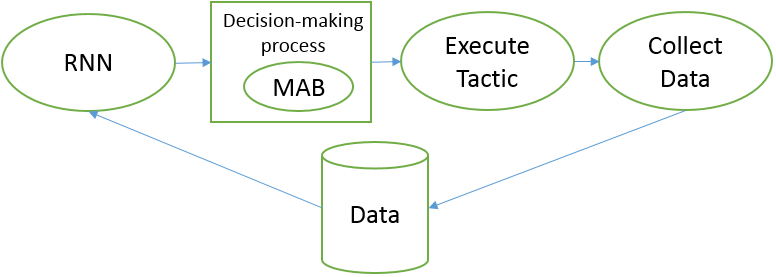
\includegraphics[width=0.8\linewidth]{images/Mab-Scratch.png}
%    \caption{TVA Process\dan{I will clean up - update}}
%    \label{fig:MABProcess}
%\end{figure}

%%%%%%%%%%%%%%%%% Start Image %%%%%%%%%%%%%%%%%%%%

\begin{figure}[h]

\begin{center}

%% Do this for right angles on connecting lines
\tikzset{
    -|/.style={to path={-| (\tikztotarget)}},
    |-/.style={to path={|- (\tikztotarget)}},
}

%% Rec, circle, rrec, arrow

\usetikzlibrary{fit, } %% Used for putting dotted box
\usetikzlibrary{calc}

\tikzstyle{line} = [draw, -latex']
\tikzstyle{arrow}=[draw, -latex] 
\
% Define block styles
\tikzstyle{line} = [draw, -latex']

\tikzstyle{circle} = [ellipse, draw, fill=white!20, text centered]

\tikzstyle{rrec} = [rectangle, draw, fill=white!20, text width=5em, text centered, rounded corners, minimum height=4em]

% Small rectangle
%\tikzstyle{smrrec} = [rectangle, draw, fill=white!20, text centered, maximum height=2em]

% Database icon
\tikzstyle{dbase} = [cylinder, draw, fill=white!20, shape border rotate=90, minimum height=3em, minimum width=1.45cm]

\scalebox{.9}{
\begin{tikzpicture}[node distance = 3.5cm, line width=.5mm]
   
    \node [dbase] (Data) {Data}; 

    \node [circle, above left of=Data, yshift=0ex, xshift=3ex, maximum height=1em, maximum width=.5em] (MAB) {MAB}; %was 3 yshift

    \node [rrec, left of=MAB] (RNN) {RNN};
    \node [rrec, right of=MAB] (Execute) {Execute Tactic(s)};
    \node [rrec, right of=Execute] (Collect) {Collect Tactic Data};

    \draw [line] (RNN) -- (MAB);
    \draw [line] (MAB) -- (Execute);
    \draw [line] (Execute) -- (Collect);
    \draw [line] (Data) -- (RNN);
    \draw [line] (Collect) -- (Data);

    \draw[black,thick] ($(MAB.north west)+(-.65,0.5)$) rectangle ($(MAB.south east)+(0.65,-0.5)$) ++(-1.3,2.2) node[below] {Decision Process};

\end{tikzpicture}
} 
\caption{Overview of TVA process}
\label{fig:TVAOverview}
\end{center}
\end{figure}

%%%%%%%%%%%%%%%%% End Image %%%%%%%%%%%%%%%%%%%%

\vspace{-5mm} % Will likely need to be adjusted

\begin{enumerate}[noitemsep]

    \item \descStep{Use RNNs to Predict Tactic Values}{Tactic attributes such as latency and cost will be predicted using the Evolutionary Exploration of Augmenting Memory Models (EXAMM) algorithm. % to evolve RNNs to predict time series data from system \hl{sensors}. 
    We will further extend \hl{?existing?} EXAMM-based methods to utilize not only mean squared error (MSE) and mean absolute error (MAE) of predictions as loss functions, but also incorporate a measure of confidence -- predicting an estimation of running standard deviation for the time series.\dan{Travis: Update}}    

    \item \descStep{Plan for Tactic Execution With Multi-Armed Bandit Approach}{The inclusion of a multi-armed bandit component will augment the system's decision-making process, and better enable the system to explore and select between multiple tactic options. The multi-armed bandit component will be especially beneficial for providing additional tactic data, especially in situations of high uncertainty/volatility and when there are little amounts of historical tactic data. %For example, consider a scenario where the system has two tactic options with equal reward, but volatile cost and latency. To enable the system to regularly gain updated cost and latency information, it is necessary to regularly `explore' the alternative tactic option to understand its updated cost information. Not exploring alternative tactic options could lead to scenarios where the system `learns' to always choose one of the tactic options, when in fact an alternative tactic option has become cheaper and/or faster. Therefore, the system would lose the opportunity to begin to utilize this alternative, more optimal tactic. 
    A challenge is to balance the `explore' and `exploit' components for the system to optimally function. While the specific implementation remains to be evaluated and determined, options include Epsilon Greedy or Upper Confidence Bound approaches. Specific domain and system requirements will heavily influence the possible influence that the multi-armed bandit component has on the system. In cases of high uncertainty or low confidence, the system may execute an appropriate \emph{uncertainty reduction tactic}~\cite{moreno2018uncertainty}
    
    
    
    
    %to exploit and explore tactic option(s) when appropriate. 
    
    
    % Briefly explain the benefits that MAB will provide.
    % Tactic predictions need further data
    
    % For example, consider a scenario where the system has two tactic options with equal reward, but volatile cost and latency. To enable the system to regularly gain updated cost and latency information
    
    
    % Not exploring alternative tactic options could lead to scenarios where the system `learns' to always choose one of the tactic options, when in fact an alternative tactic option has become cheaper and/or faster. Therefore, the system would lose the opportunity to begin to utilize this alternative, more optimal tactic. 
    
    
    }
    
    %The system will plan for tactic execution(s) using a multi-armed bandit component. This will enable the system to effectively perform, while also accounting for volatility, uncertainty and a lack of empirical data. While the specific implementation remains to be evaluated and determined, several initial options include Epsilon Greedy or Upper Confidence Bound approaches. Specific domain and system requirements will heavily influence the possible `exploration' that is conducted by the selected multi-armed bandit approach. In cases of high uncertainty or low confidence, the system may execute an appropriate \emph{uncertainty reduction tactic}~\cite{moreno2018uncertainty}.}
    
    %Plan for Tactic Execution Using Multi-Armed Bandit Approach}{Existing knowledge, system rules and the results from the RNN model will be incorporated into our decision-making process which a significant Multi-Armed Bandit component. This will enable the system to not only account for the predicted tactic, but also account for predicted tactic confidence and variance. This multi-armed bandit approach, coupled with the use of evolutionary RNNs will enable the system to most appropriately function in new and uncontrolled areas, and especially those with volatile or small amounts of historical data.\todo{work on this section}}
    
    % Help in scenarios where little information is known
    % Assist when there isn't much confidence about a predicted value
    % ? Which MAB process will we use.
    
    % Combine with the RNNs results along with system/domain-specific requirements to determine the most appropriate tactics to implement.
    
    % Provide more specifics about how we plan to use MABs
    
    
    
%    \item \descStep{Plan for Tactic Execution}{The Multi-Armed Bandit component will determine the most appropriate tactic(s) to execute.}
    
    
    \item \descStep{Execute Tactics}{Tactics are executed according to defined plan.}



    \item \descStep{Collect Tactic Data}{System sensors record the amount of time and cost required to execute the adaptation tactic(s). Other relevant time series data will also be collected by the system throughout its operation. This data will also be included in future tactic-based predictions.}




%    \item \descStep{Collect tactic values}{XXXXX}
%    \item \descStep{Make prediction for latency, cost, \etc}{XXXXX}
%    \item \descStep{Put prediction back into decision-making process}{XXXXX}



\end{enumerate}



%%%%%%%%%%%%%%%%%%%%%%%%%%%%%%%%%

%Our proposed TVA solution will benefit a variety of autonomous systems through its easy integration into a diverse forms of self-adaptive processes. (HOW)..... 


%TVA will enable autonomous to better react to tactic volatility using the following processes:





%Can impact adaptation tactics, along with adaptation strategies which are predefined compositions of adaptation tactics~\cite{moreno2017adaptation}.



%decision trees built out of adaptation tactics~\cite{moreno2017adaptation}.

%\begin{enumerate}[noitemsep]

%    \item \descStep{Collect tactic values}{XXXXX}
%    \item \descStep{Make prediction for latency, cost, \etc}{XXXXX}
%    \item \descStep{Put prediction back into decision-making process}{XXXXX}
%    \item \descStep{XXX}{XXXXX}


%\end{enumerate}



% DK: I think that these are good, but are also a bit too technical and miss several important details.
%Our TVA process will consist of several primary phases which are described below:

%\begin{enumerate}[noitemsep]

%\item \descStep{Predict Tactic Volatility}{We will use the Evolutionary Exploration of Augmenting Memory Models (EXAMM) algorithm to evolve RNNs to predict time series data from system \hl{sensors}. We will further extend EXAMM to utilize not only mean squared error (MSE) and mean absolute error (MAE) of predictions as loss functions, but also incorporate a measure of confidence -- predicting an estimation of running standard deviation for the time series.}

%\item \descStep{Bootstraping Trained RNNs to New Scenarios and Data}{We will investigate the use of using previously trained RNNs and evolving them to quickly predict new parameters with limited available data, for example, if a new sensor system becomes available; or re-evolve a network if sensors are damaged and become unavailable.\dan{we should add in a few words how this fits into TVA better.}}

%\item \descStep{Incorporate predictions into decision-making process}{The anticipated tactic volatility values will be incorporated into the decision-making processes in several ways. The estimated tactic values can be used to make more accurate predictions for what the attained \emph{utility} of a specific tactic will be. This can in turn, impact the expected utility of the larger \emph{adaptation strategies} that the system may take. The anticipated tactic latency times will enable the system to more accurately determine when tactics should be proactively began to ensure that they are ready when needed, thus improving system effectiveness and reducing cost due to the system realizing less waste with tactics enacted before they are needed. The latency values will also be used by the system to make more informed decisions about how different tactics and adaptation strategies will impact concurrent and subsequent tactics and adaptation strategies.}



%The calculated confidence and variance of parameters in the tactic predictions can provide even further data points that the system can incorporate into its decision-making process. For example, if a tactic prediction has a low amount of confidence, the system could choose to execute an \emph{uncertainty reduction tactic}~\cite{moreno2018uncertainty} to potentially provide a more accurate prediction.\dan{move}



%The estimated tactic values will be included in the system's \emph{utility} equation which is often used to guide the system's actions and the decisions-made by the system. The estimated values will also be \hl{compared} with the specifications defined in the SLA to enable the system to act more proactively when necessary to ensure that the specifications defined in the SLA are adhered to.\dan{rewrite this}\dan{make sure that this is all accurate}}

% DK: Be sure that I am using adaptation tactic and adaptation strategy correctly here.


%The estimated tactic values will be included in the system's decision-making process, enabling it to make more informed decisions leading to more optimal outcomes.


%% DK: I am not sure that this step is actually needed since it is kind of explained in the previous step
%\item \textbf{Perform system operations using predictions: }The input values will enable the system to make more appropriate and informed actions, thus supporting it in dynamic and volatile environments. \dan{rewrite this}
	
%\end{enumerate}

%\dan{ALL: Does this provide enough information/confidence for how this will actually work?}



% Provide the reader confidence in how all of this comes together

% Process of how TVA works collected tactic information, learning, prediction, action. 
%   Where is it integrated to in the MAPE-K control loop. 

% Provide a lot of confidence for how it will be integrated into the self-adaptive process
% Talk about why RNN is the most appropriate solution here. Provide confidence. Also, discuss a bit about how RNN works

% Mention how it will integrate into a variety of autonomous systems (either here or in another section of the paper)



% In systems that do not directly utilize a SLA, the improved tactic estimations can still be used to benefit the decision-making process of these systems by providing more informed and accurate tactic attribute values. Future work should be conducted to examine precisely how our TVA process can be incorporated into these systems and determine the benefits that they will have.



%\subsection{--- ML and how it will fit into this project ----}

%\dan{Travis/Qi/Alex: this is your section}

% What is the process we will use
% Why will it be the most effective from a technical perspective. 
% What are some things that make it innovative/interesting.



% DK: Provide the reader confidence in why the ML techniques we are choosing will be proper. Don't be afraid to be a bit innovative here.





% DK: Probably cut down on this space a bit more in the event space is needed. I think that this section is less important that most of the others.
\subsection{Evaluation Process}

% Describe how it will be evaluated using different tools, different data sets. Make the reader confident in the need to create our own dataset.

We will evaluate our proposed TVA processes against the defined objectives using our created dataset containing real-world tactic volatility using statistical evaluations such as R and MatLaB, and in the existing simulation environments SWIM~\cite{moreno2018swim} and DARTSIM~\cite{MorenoDART2019}. %\dan{Add in how R, MatLab will be used.}
To support the evaluation of TVA, enhancements to DARTSim and SWIM will include support for volatile data, additional scenarios, and new adaptation tactics and strategies. The effectiveness of our proposed TVA solution will be evaluated using several metrics including: (I) Expected vs realized utility (II) Ability to complete defined mission/system critical functionality when encountering unexpected volatility and when operating in new environments (III) Ability of TVA to assist the system's ability to execute concurrent and subsequent adaptation tactics and strategies (IV) Speed of learning..... ???   .\dan{What more can we add to these?}

%To evaluate our work, we will utilize several scenarios, including the cloud-based example described in Section~\ref{sec: motivatingexample} and the UAV scenario provided in DARTSim.






%The effectivness to:
%-   execute si


% How and why we will need to modify the tools
% What metrics will we use evaluate the techniques.
% What scenarios will we use (use the existing cloud-based or come up with a military scenario)
 



% Train in different environments
% Cut out sensors
% Different systems

 



\todo{How will we evaluate the ML portion}

We will evaluate various multi-armed bandit solutions (\eg Epsilon-Greedy, Upper Confidence Bound, Bayesian) to assess their effectiveness in various autonomous environments and scenarios.
% DK: This section is not needed, so we can likely remove it if space is an issue
\section{Summary of Recent Work}\vspace{-2mm}

% Cut this down/clean it up
We are the first to make tactic volatility a first-class concern in the self-adaptive decision-making process~\cite{Krutz_ase_2019}. Previous works have examined tactic latency and cost, demonstrating the importance of accounting for these during the self-adaptive process~\cite{Moreno:2018:FED:3208359.3149180, 7573126, moreno2017adaptation, moreno2015proactive, Jung:2009:CAE:1813355.1813367}. However, existing works merely consider these attributes to be static values and do not enable the system to learn and account for tactic volatility.  



%\dan{Describe a bit of what RNNs/the adopted learning method are used for - Keep this to a paragraph or so - Also mention a bit about MABs}

% Tactics and Latency in self-adaptive systems







% DK: Maybe change this title
\section{Required Government Support} % Required Section
No government support in the form of facilities, equipment, demonstration sites, test ranges, software, personnel or materials is anticipated to be required to successfully execute this research.
%\vspace{-8mm}
\section{Cost Estimate} % Required Section
\vspace{-2mm}
% DK: Make this a bit more detailed

%~600K

The total budget for the three year project is \$250k/yr for a total cost of \$750k. This budget will include: I) PhD student support II) Summer support for the project team  III) Equipment (IV) Travel for dissemination and collaboration. %A broad overview of our funding plan is shown in Table~\ref{table:budget}. %\todo{update all of this}

% 1.2


%\begin{table}[h]
%\begin{center}
%\caption{Budget Summary}
%\label{table:budget}


% 350/yr?

%\begin{tabular}{ c | c | c  }
			
%  \textbf{Y1} & \textbf{Y2} & \textbf{Y3} \\   \hline
%  250k & 250k & 250k \\
%   \end{tabular}
%  \end{center}
%\end{table}




%and have collectively authored more than \hl{XXX} works, many of which have appeared in top-tier venues. 
%PI Krutz was a 2018 Research Fellow for the AFRL working in the area of artificial intelligence. Project members include: %A broad overview of our funding plan is shown in Table~\ref{table:budget}.


%\begin{table}[h]
%\begin{center}
%\caption{Budget Summary}
%\label{table:budget}

%\begin{tabular}{ c | c | c  }
			
%  \textbf{Y1} & \textbf{Y2} & \textbf{Y3} \\   \hline
%  175k & 175k & 175k \\
%   \end{tabular}
%  \end{center}
%\end{table}


%   ? What is the typical budget
% 1 PhD student supervised by Krutz/Qi, the other by Travis/Alex (2 total)

%\vspace{-5mm}
% Not sure we should have this section
%\subsection*{Project Team}








%%%%%%%%%%%%%%%%%%%%%%%%%%%%%%%%

\label{lastpage}
\cleardoublepage


\appendix


%% DK: Put onto a different page since it does not count against the page limit
\setcounter{page}{1}

\cfoot{\thepage}
\pagenumbering{roman}



%%%%%%%%%%%%%%%%%%
\newpage

\section*{Addendum} % (Not to exceed one page) This page is in addition to the 5 other pages


\newcommand{\AuthorInfo}[3]{\noindent \textbf{#1  #2} #3}



The project team has a demonstrated record of success in collaborating to successfully execute DOD funded projects, along with disseminating their research together in top-tier publications.\\

\AuthorInfo{PI}{Daniel E. Krutz}{is an Assistant Professor at Rochester Institute of Technology, Department of Software Engineering. Krutz the Director of the Autonomy, WARfare, and Engineering (AWARE) Lab\footnote{\url{http://aware.rit.edu}}, which supports several externally funded projects for the NSF, NSA and the DOD. His research interests include Self-adaptive systems, decision support systems and computing education. Krutz is the author of over 32 peer reviewed publications, many of which have appeared in top-tier venues. In 2018 Krutz was a research faculty fellowship at the US Air Force Research Laboratory (AFRL), working in the area of autonomy/AI.}\\


\AuthorInfo{Co-PI}{Qi Yu}{Stuff}\\


\AuthorInfo{Co-PI}{Travis Desell}{Stuff}\\


\AuthorInfo{Co-PI}{Alex Orobia}{Stuff}




%%%%%%%%%%%%%%%%%





%% I think the appendix goes before the bib. Otherwise, I could see people missing it
\newpage
\pagebreak
\addcontentsline{toc}{section}{References}
\bibliographystyle{plain}
\bibliography{refs}

\end{document}


%% Possible DARPA program
%   https://www.darpa.mil/program/assured-autonomy






%%%%%%%%%%
- In cases where data is unknown, use MAB

